\documentclass[tikz,border=7pt]{standalone}
\usepackage{amsmath}
\usepackage{xcolor}
\usetikzlibrary{arrows.meta,positioning,calc,fit}

% Reproducible paper-style source for assets/diagrams/han-agents.svg
% Build from this directory:
%   pdflatex -interaction=nonstopmode -halt-on-error han-agents.tex
%   pdftocairo -svg han-agents.pdf han-agents.svg

\definecolor{ink}{HTML}{203746}
\definecolor{muted}{HTML}{647783}
\definecolor{line}{HTML}{AFC2CE}
\definecolor{panel}{HTML}{F8FAFB}
\definecolor{blue1}{HTML}{E8F1F6}
\definecolor{blue2}{HTML}{C9DDE8}
\definecolor{blue4}{HTML}{4D86A4}
\definecolor{teal}{HTML}{2F7D78}
\definecolor{tealfill}{HTML}{E7F3F1}
\definecolor{orange}{HTML}{C9743A}
\definecolor{orangefill}{HTML}{F8EBDD}
\definecolor{gold}{HTML}{9A7A2C}
\definecolor{goldfill}{HTML}{F6F0DE}
\definecolor{green}{HTML}{4D7C59}
\definecolor{greenfill}{HTML}{EAF2EC}

\tikzset{
  >={Stealth[length=2.1mm,width=1.5mm]},
  flow/.style={->, draw=muted, line width=0.9pt},
  strongflow/.style={->, draw=blue4, line width=1.1pt},
  feedback/.style={->, draw=orange, line width=1.0pt},
  panelbox/.style={draw=line, fill=panel, rounded corners=2.0mm, line width=0.65pt},
  layer/.style={draw=line, fill=white, rounded corners=1.5mm, line width=0.7pt,
                minimum width=3.25cm, minimum height=1.42cm, align=center},
  process/.style={draw=line, fill=white, rounded corners=1.7mm, line width=0.8pt,
                  minimum width=3.15cm, minimum height=1.30cm, align=center},
  title/.style={font=\sffamily\bfseries\large, text=ink},
  section/.style={font=\sffamily\bfseries\small, text=muted},
  label/.style={font=\sffamily\bfseries\small, text=ink},
  sub/.style={font=\sffamily\scriptsize, text=muted, align=center},
  tiny/.style={font=\sffamily\scriptsize, text=ink, align=center},
}

\begin{document}
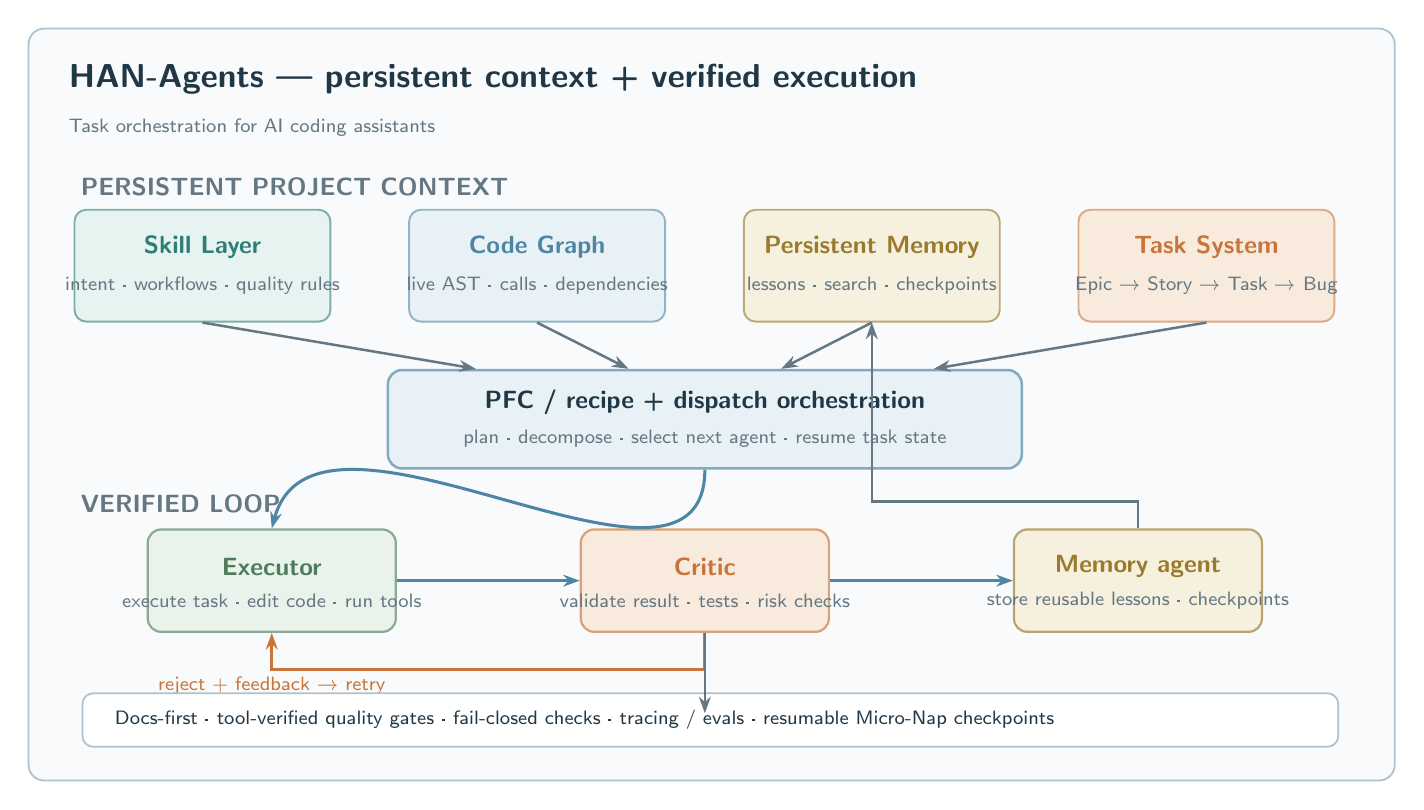
\begin{tikzpicture}[x=1cm,y=1cm]

% Canvas ----------------------------------------------------------------------
\node[panelbox, minimum width=17.35cm, minimum height=9.55cm, anchor=south west] (canvas) at (0,0) {};
\node[title, anchor=north west] at ([xshift=4mm,yshift=-3.4mm]canvas.north west)
  {HAN-Agents — persistent context + verified execution};
\node[sub, anchor=north west] at ([xshift=4mm,yshift=-10.3mm]canvas.north west)
  {Task orchestration for AI coding assistants};

% Persistent context -----------------------------------------------------------
\node[section, anchor=west] at (0.55,7.55) {PERSISTENT PROJECT CONTEXT};

\node[layer, fill=tealfill, draw=teal!62] (skill) at (2.22,6.55) {};
\node[label, text=teal] at ($(skill.center)+(0,0.24)$) {Skill Layer};
\node[sub] at ($(skill.center)+(0,-0.25)$) {intent · workflows · quality rules};

\node[layer, fill=blue1, draw=blue4!62] (graph) at (6.47,6.55) {};
\node[label, text=blue4] at ($(graph.center)+(0,0.24)$) {Code Graph};
\node[sub] at ($(graph.center)+(0,-0.25)$) {live AST · calls · dependencies};

\node[layer, fill=goldfill, draw=gold!65] (memory) at (10.72,6.55) {};
\node[label, text=gold] at ($(memory.center)+(0,0.24)$) {Persistent Memory};
\node[sub] at ($(memory.center)+(0,-0.25)$) {lessons · search · checkpoints};

\node[layer, fill=orangefill, draw=orange!62] (tasks) at (14.97,6.55) {};
\node[label, text=orange] at ($(tasks.center)+(0,0.24)$) {Task System};
\node[sub] at ($(tasks.center)+(0,-0.25)$) {Epic → Story → Task → Bug};

% Orchestration core -----------------------------------------------------------
\node[draw=blue4!70, fill=blue1, rounded corners=1.8mm, line width=0.9pt,
      minimum width=8.05cm, minimum height=1.25cm, align=center] (orch) at (8.60,4.60) {};
\node[label] at ($(orch.center)+(0,0.22)$) {PFC / recipe + dispatch orchestration};
\node[sub] at ($(orch.center)+(0,-0.25)$) {plan · decompose · select next agent · resume task state};

\draw[flow] (skill.south) -- ($(orch.north west)!0.14!(orch.north east)$);
\draw[flow] (graph.south) -- ($(orch.north west)!0.38!(orch.north east)$);
\draw[flow] (memory.south) -- ($(orch.north west)!0.62!(orch.north east)$);
\draw[flow] (tasks.south) -- ($(orch.north west)!0.86!(orch.north east)$);

% Verified execution loop ------------------------------------------------------
\node[section, anchor=west] at (0.55,3.52) {VERIFIED LOOP};

\node[process, fill=greenfill, draw=green!65] (exec) at (3.10,2.55) {};
\node[label, text=green] at ($(exec.center)+(0,0.18)$) {Executor};
\node[sub] at ($(exec.center)+(0,-0.25)$) {execute task · edit code · run tools};

\node[process, fill=orangefill, draw=orange!68] (critic) at (8.60,2.55) {};
\node[label, text=orange] at ($(critic.center)+(0,0.18)$) {Critic};
\node[sub] at ($(critic.center)+(0,-0.25)$) {validate result · tests · risk checks};

\node[process, fill=goldfill, draw=gold!68] (memagent) at (14.10,2.55) {};
\node[label, text=gold] at ($(memagent.center)+(0,0.18)$) {Memory agent};
\node[sub] at ($(memagent.center)+(0,-0.25)$) {store reusable lessons · checkpoints};

\draw[strongflow] (orch.south) to[out=-90,in=75] (exec.north);
\draw[strongflow] (exec.east) -- (critic.west);
\draw[strongflow] (critic.east) -- (memagent.west);

% Reject / retry feedback
\draw[feedback] (critic.south) -- ++(0,-0.46) -| node[pos=0.54,below,sub,text=orange] {reject + feedback → retry} (exec.south);

% Accepted lessons re-enter persistent memory
\draw[flow] (memagent.north) -- ++(0,0.34) -| (memory.south);

% Quality / observability strip ------------------------------------------------
\node[draw=line, fill=white, rounded corners=1.4mm, line width=0.65pt,
      minimum width=15.95cm, minimum height=0.68cm] (gate) at (8.67,0.78) {};
\node[tiny, anchor=west] at ([xshift=3mm]gate.west)
  {Docs-first  ·  tool-verified quality gates  ·  fail-closed checks  ·  tracing / evals  ·  resumable Micro-Nap checkpoints};

\draw[flow] (critic.south) -- ++(0,-1.02);

\end{tikzpicture}
\end{document}
